% !TeX spellcheck = en_US
\section{Quality Impairments}
\label{sec:415_quality_impairments}
\subsection{Recording Degradations}
Major degradations occurring in \ac{UGV} are camera shakes, harmful occlusions, and camera misalignments.
\subsubsection{Camera Shakes}
Due to the lack of a stabilizing tripod, small, uncontrolled movements by the recording user can lead to undesired motions captured by the video.
If these motions occur continuously with varying motion directions, they are named camera shakes.
Intended motions of the camera include tilting and panning.
In contrast to a camera shake, these intended forms of motion do not show repeated direction changes~\cite{Ward2003}.

Characteristics of this degradation include the amplitude, the direction, the speed, as well as the duration of a camera shake.
These characteristics are analyzed concerning their impact on the quality of a subjective video quality assessment.
The definition of the characteristics is as follows:
\begin{itemize}
	\item \emph{Amplitude}: The amplitude determines the amount of movement into a certain direction. 
	It is measured in the portion of a frame as a percentage of the video frame added to the top and bottom (or left and right).
	\item \emph{Direction:} Distinction on whether the shake is performed along the horizontal or vertical axis.  
	\item \emph{Speed of shake:} A relative measure of the percentage of a video frame skipped in one second of video. 
	\item \emph{Duration:} The delta of playback points in time between the start and the end of a camera shake in a single video sequence.
\end{itemize}

\subsubsection{Harmful Occlusions}
Many occlusions are not perceived as distortions as they are part of a scene.
In cases when a foreground object crosses the line of sight between a recording device and a background object the user is interested in (\ac{RoI}), the occlusion becomes distracting. 
Thus, \emph{harmful occlusions} limit the possibility to record video content. 
Relevant characteristics of harmful occlusions include:
\begin{itemize}
	\item \emph{Size:} The percentage of the video frame that is occluded. 
	\item \emph{Position:} In which part of the video frame does the harmful occlusion occur? The occlusion may appear at the top or the bottom of the video frame.
	It may arise from the left or the right of the video frame. 
	\item \emph{Duration:} The delta in playback time between the points in time a harmful occlusion appears and disappears in a sequence.
\end{itemize}

\subsubsection{Camera Misalignment}
\emph{Misalignment of the camera} represents an event in which the camera is not focusing on the commonly agreed \ac{RoI}, e.g., the stage during a concert.
Misalignments start from slightly drifting away from keeping the main actions in the center of a recorded sequence.

In its worst form, the recording does not capture the \ac{RoI} at all. 
We evaluate different misalignment types, which vary in terms of their direction, the misalignment from the \ac{RoI} of a frame ("Percentage"), and their duration. 
The characteristics are described as:
\begin{itemize}
	\item \emph{Direction:} The direction describes whether the camera is misaligned to the left, right, top, or bottom of a video frame.
	\item \emph{Percentage:} The amount of misalignment measured as the percentage of the total video frame no longer perceivable due to the misalignment.
	\item \emph{Duration:} The delta between the start of a camera misalignment and its end in a single video sequence.
\end{itemize}
\subsection{Recording Position}
Different video views of the scene can be distinguished regarding the geographic position and the orientation of the recording device.
Whereas the quality models for the assessment of the \emph{recording quality} can be applied to any \ac{UGV}, the models created for the \emph{recording position} assume that all video views capture a common \ac{AoI}. 
To map the position relative to a single event, each position can be described in relation to the \ac{PoI} as the reference point.

This position can be acquired using location providers on today's recording devices, including \ac{GPS}.
In the proposed models, this position is simplified to a two-dimensional model.
The \ac{PoI} can, for example, be the stage in a concert hall, in which performers act.
The distance is being measured in meters by transforming the \ac{GPS} coordinates to a \ac{UTM} model.
Distances can be classified into shot types: close-up, medium, medium-long, and long shots~\cite{Bowen2013}.
These shot types were introduced in Section~\ref{sec:240_VideoViews}.
This classification allows an easier comparison than the nominal distance in meters as the latter must be assessed in relation to the size of the \ac{PoI} and the objects that are of interest.

Besides the shot types, the distance and the angle to a \ac{PoI} play a major role in the perceived quality.
Here, a frontal face capture is depicted by $0\degree$ whereas $90\degree$ shows a recording from the side of a stage.
The angles of the orientations are measured in $10\degree$ steps from the origin with $0\degree$ to $90\degree$.
The assumption is that no sensible recording can be created beyond the $90\degree$ angle. 
Figure~\ref{fig:420_position_angle} gives an idea of the concepts of distance and angle.
A traditional, proscenium show stage is assumed. 
For central staging scenarios a rectangular stage is assumed where each side is evaluated individually.
\begin{figure}[h!]
	\centering
	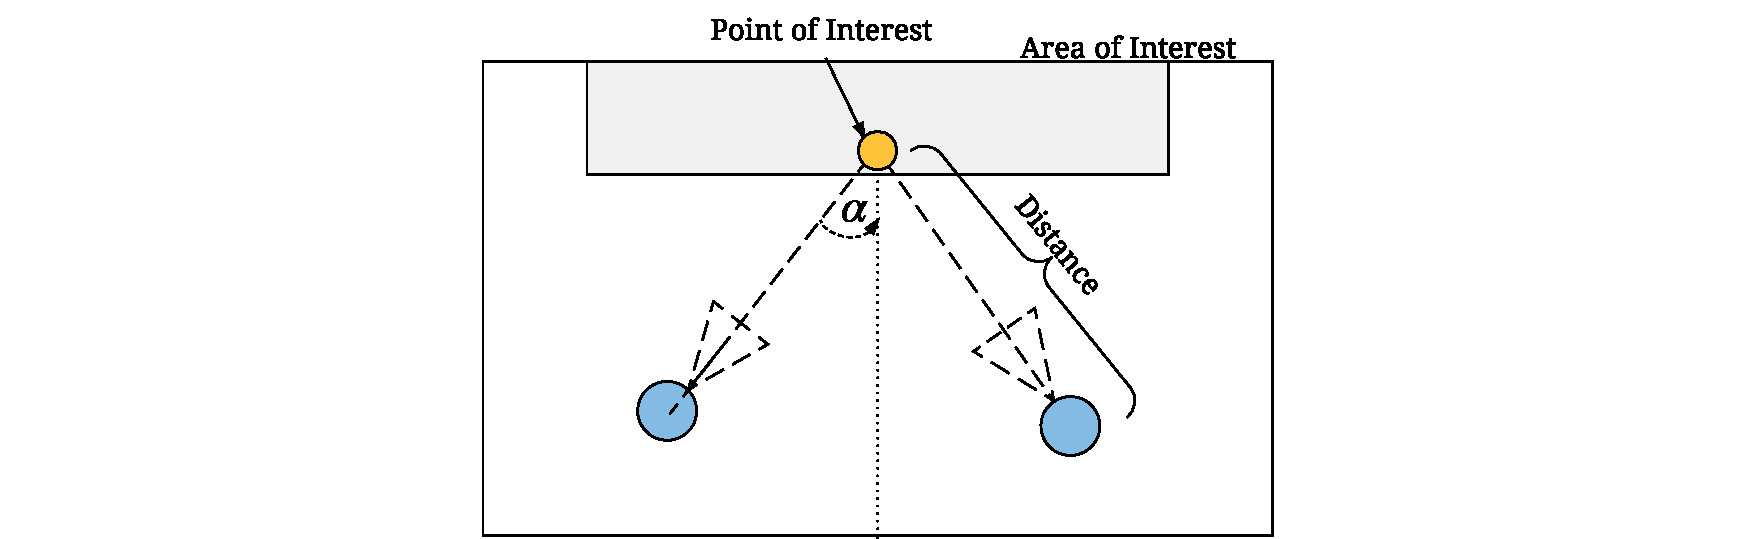
\includegraphics[width=\linewidth]{gfx/400_UGV_Quality/position_angle}
	\caption[Illustration on measured attributes of a recording position]{Illustration of measured attributes of a recording position: distance and angle.}
	\label{fig:420_position_angle}
\end{figure}

\section{Approach for Conducting User Studies}
\label{sec:420_approach_recording}
The quality models are generated using large-scale user studies.
To achieve accurate models for the range of various degradations and their characteristics, the concept of crowdsourcing is used. 
Lab experiments ensure the validity of the generated models, as they are conducted in a controlled environment.
A comparable \ac{UI} and the same rating methodology and experiment setup were used for the studies. 

The studies are conducted following the principles defined by \ac{ITU}-R BT.500~\cite{ITU-R2012} and \ac{ITU}-T P.910~\cite{ITU-J2008} for making subjective video quality assessments.
All users watch multiple video sequences of a length of 8 seconds to 12 seconds.
An \ac{SSCQS} is used, which allows users to assess each video individually.
Details on the fundamentals for subjective studies are given in Section~\ref{sec:210_subjective_quality}.
\subsection{Crowdsourcing}
Ratings for quality models are gathered in large-scale studies using the concept of crowdsourcing.
It is applied in a manner so that the quality assessments are distributed to a random set of people mediated by a crowdsourcing platform.
Users rate the quality of impaired video sequences in relation to a reference.
All users are compensated for their work.
The crowdsourcing mediator Microworkers\footnote{www.microworkers.com; Visited on: 09/24/2016} provides the respective crowdworkers.
The evaluations leverage a web-based system, which allows to play back a stall-free video segments and offers users to rate the shown video sequences. 
\subsubsection{Recording Quality}
The recording quality assessment consists of 16 crowdsourcing runs with an average of 101 workers each. 
The crowdsourcing task includes to watch six video sequences in random order, including an unknown reference video. 
Users rate the video sequence quality on the \ac{SSCQS}~\cite{ITU-R2012}.
Thus, the task of each worker is to detect and rate degradations in the video sequences.
Tasks are clustered in so-called campaigns.
Each campaign represents a distinct set of video clips from one specific genre, which allows us to calculate consistent results under similar conditions. 
A qualification task is designed in which multiple degradations had to be found and rated. 
These qualification tasks train the workers and provide quick feedback on the reliability of the users.
Only workers who successfully completed the qualification task are invited to participate in the evaluation. 
These workers are granted access to campaigns for assessing both the recording quality and the recording position.
\subsubsection{Recording Position}
The aim of this experiment is to build accurate models on the impact of the recording position on the perceived quality.
Thus, the crowdsourcing experiment asks workers to watch eight randomly ordered video sequences of the same event.
The task of the workers is to judge the perceived video quality of each sequence using the \ac{SSCQS} recommended by the \ac{ITU}~\cite{ITU-R2012}. 
 
Each campaign represents a distinct set of video sequences from one of the genres: "sports," "music," "show," or "scenery". 
Each scene is recorded from different distances and angles that result in eight evaluated events and 79 sequences. 
The order of the video sequences is randomly selected for each user.
In combination with a large number of workers and tests, this leads to a reduced biasing of the subjective ratings. 
In total, 451 workers watch and rate the video sequences, resulting in 3160 ratings. 
\subsubsection{Lab Validation}
The lab experiments ensure that crowdsourced quality models are valid even in a controlled environment, since in crowdsourcing experiments, environmental conditions and a subject's health condition cannot be controlled. 
Lab experiments are conducted under our supervision and follow the recommendations of the \ac{ITU}~\cite{ITU-R2012} regarding display size and lighting conditions.
After playback of a video sequence, a five-second rating time is given.
No data from the training session or qualification test is used for the final results. % or evaluated in any other manner. 

Lab experiments for the recording quality assessment consist of 16 test subjects, and 15 test subjects are recruited for assessing the recording location. 
A well-illuminated room with blinded windows is used in conjunction with a 42-inch display with a \ac{720p} resolution.
As lab experiments are costly, only a limited set of characteristic combinations, e.g., the impact of the speed of camera shakes on the perceived quality, are evaluated.
\subsection{Evaluated Videos}
\label{sec:420_approach_evaluated_videos}
\subsubsection{Recording Quality}
The videos included sequences from different datasets and from different genres. 
Here, the high-definition video dataset~\cite{Keimel2010} of TU M\"unchen as well as the JIKU video dataset~\cite{Saini2013} provide different high-quality video sequences. 
\begin{figure}[htb]
	\centering
	\subfloat[]{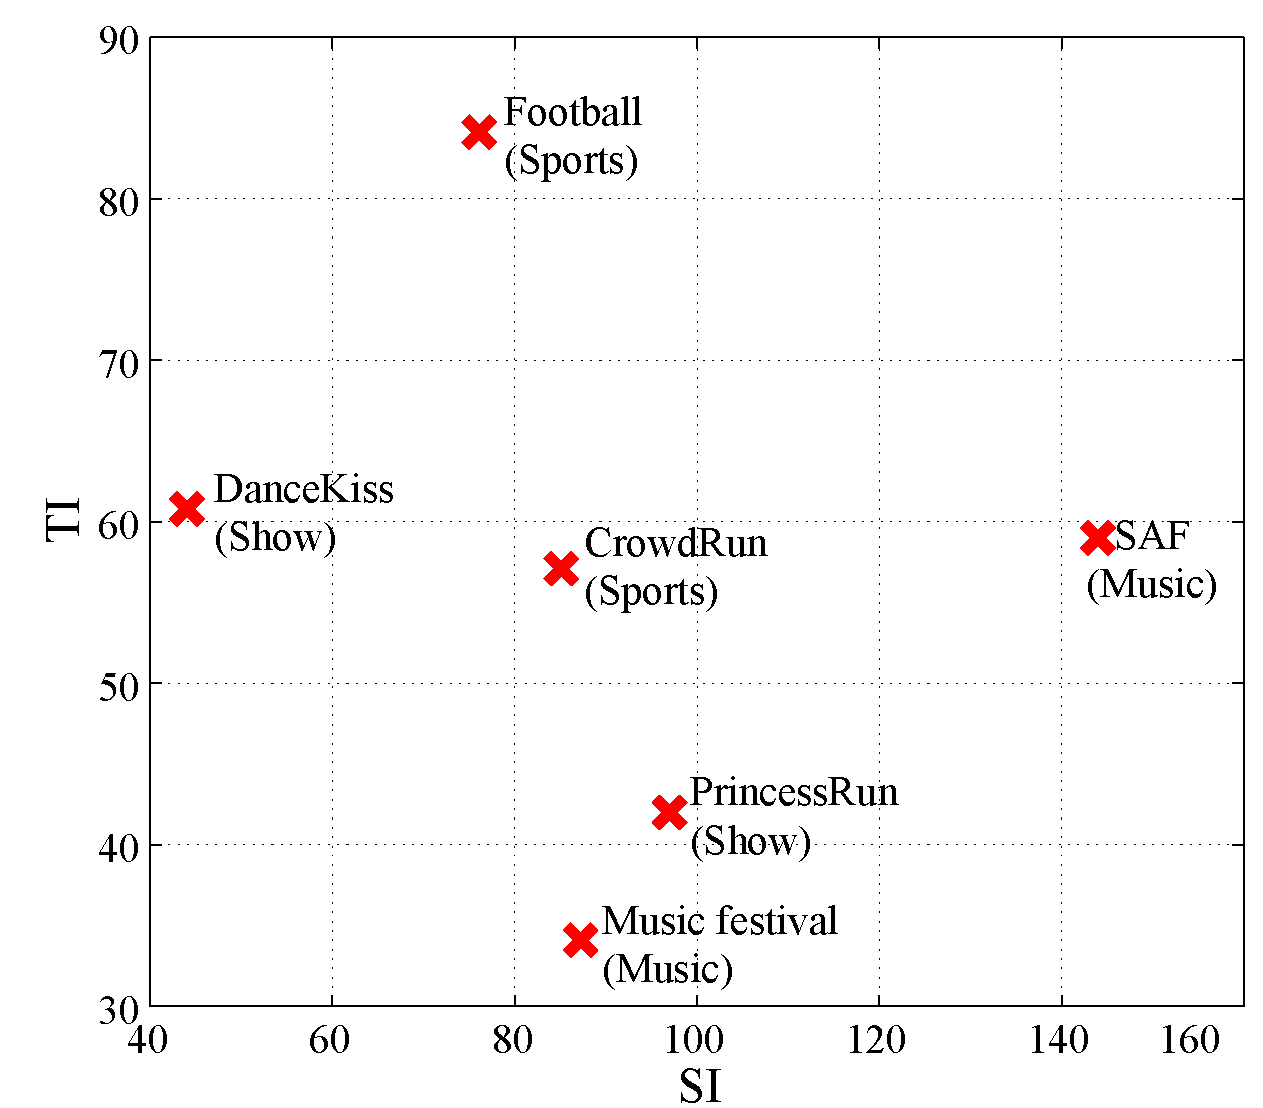
\includegraphics[width=0.55\linewidth]{gfx/400_UGV_Quality/siti_plot}}\\	
	\caption[SI and TI for the recording degradation video dataset.]{SI and TI for the video sequences used for assessing the impact of recording degradations on the perceived quality.}
	\label{fig:420_siti_plot}
\end{figure}
Also, 349 of the video sequences are recorded during a music festival and football matches in Darmstadt and Frankfurt. 
The JIKU dataset is a realistic set of recordings of a live event that shows degradations, such as shakes or occlusions. 
As the JIKU dataset does not include all degradations in the required fine granularity, videos from the TU M\"unchen dataset are artificially impaired. 
Traces of potential shakes or occurrences of occlusions were retrieved from the JIKU dataset.
The \ac{720p} resolution versions of the TU M\"unchen dataset allow using lossless video information as well as comparisons between the reference and the impaired video sequences. 
All video sequences have a duration of 9 to 12 seconds.
Videos from the TU M\"unchen dataset are re-encoded in a lossless manner using H.264/\ac{AVC} high 4:4:4 profile. 
All videos are sampled down to a resolution of \ac{4CIF} for the crowdsourcing experiments. 
In total, 1090 video clips from the three genres of sports, entertainment (no music) and music are used.
The videos include different levels of structure and motions. 
The average \ac{SI} and the \ac{TI}~\cite{ITU-J2008} characteristics of all reference videos are presented in Figure~\ref{fig:420_siti_plot}.
\ac{SI} depicts the structural complexity of a video sequence represented by the edges present in the frames of the sequence.
\ac{TI} gives the amount of motion in a video sequence, described as the displacement of edges in consecutive video frames.
Details on the calculation of \ac{SI} and \ac{TI} are given in Section~\ref{sec:630_autocompose}. 
\subsubsection{Recording Position}
For the recording position assessment, new video sequences had to be created by recording different events in parallel.
The videos are recorded during a motorbike race and a soccer game (genre: "sports"), a concert (genre: "music"), two entertainment events (genre: "show"), and points of interest in different German cities (genre: "scenery"). 
\begin{figure}[!htb]
	\begin{tabular}{ccc}
		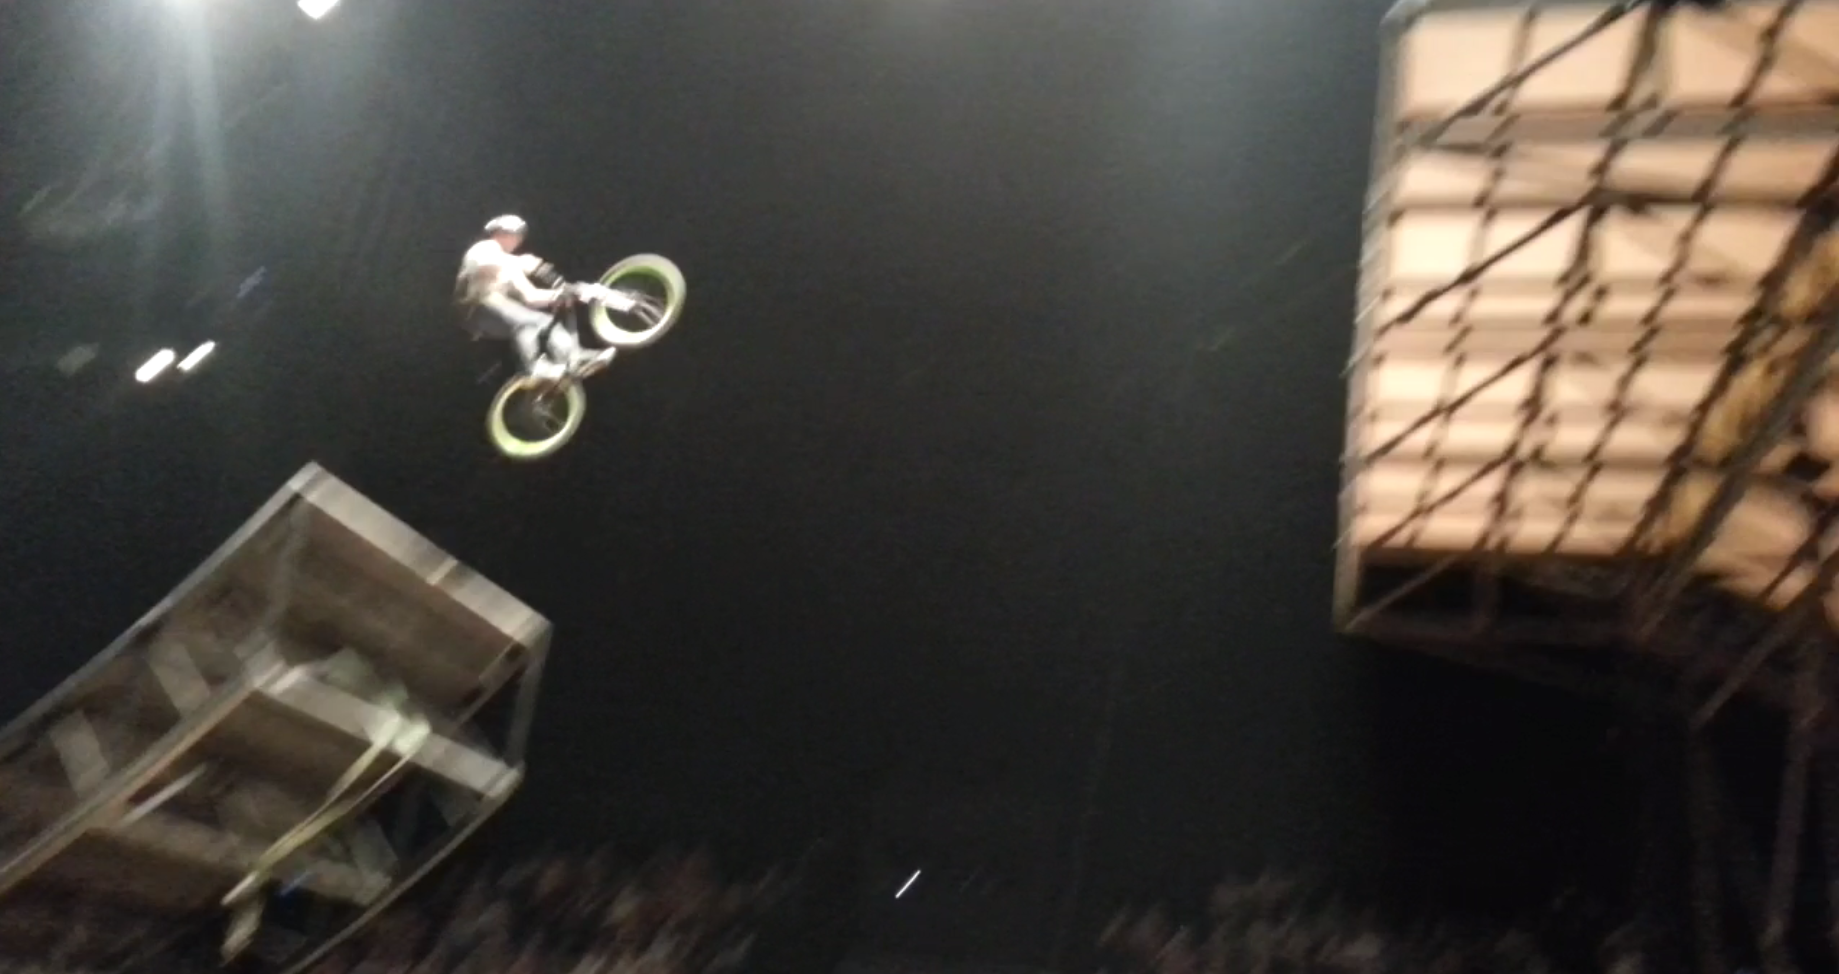
\includegraphics[width=.33\textwidth]{./gfx/400_UGV_Quality/Video_Frames/Bike1} &
		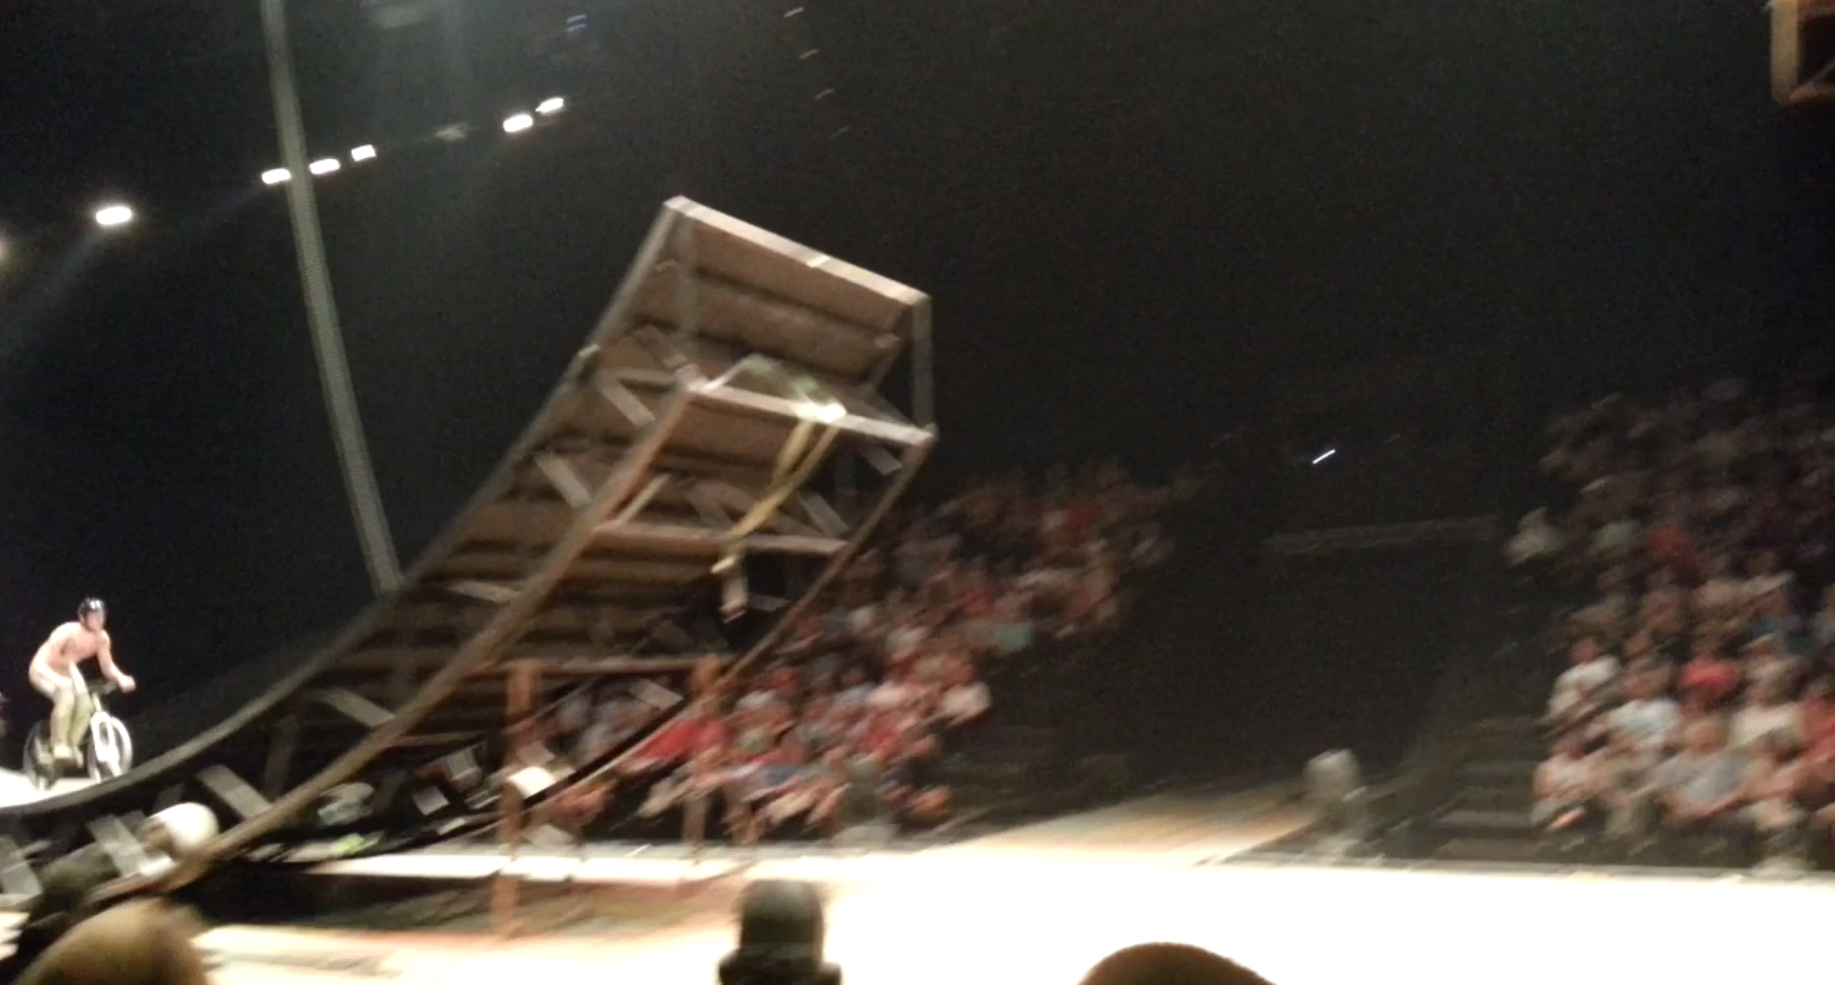
\includegraphics[width=.325\textwidth]{./gfx/400_UGV_Quality/Video_Frames/Bike2} &
		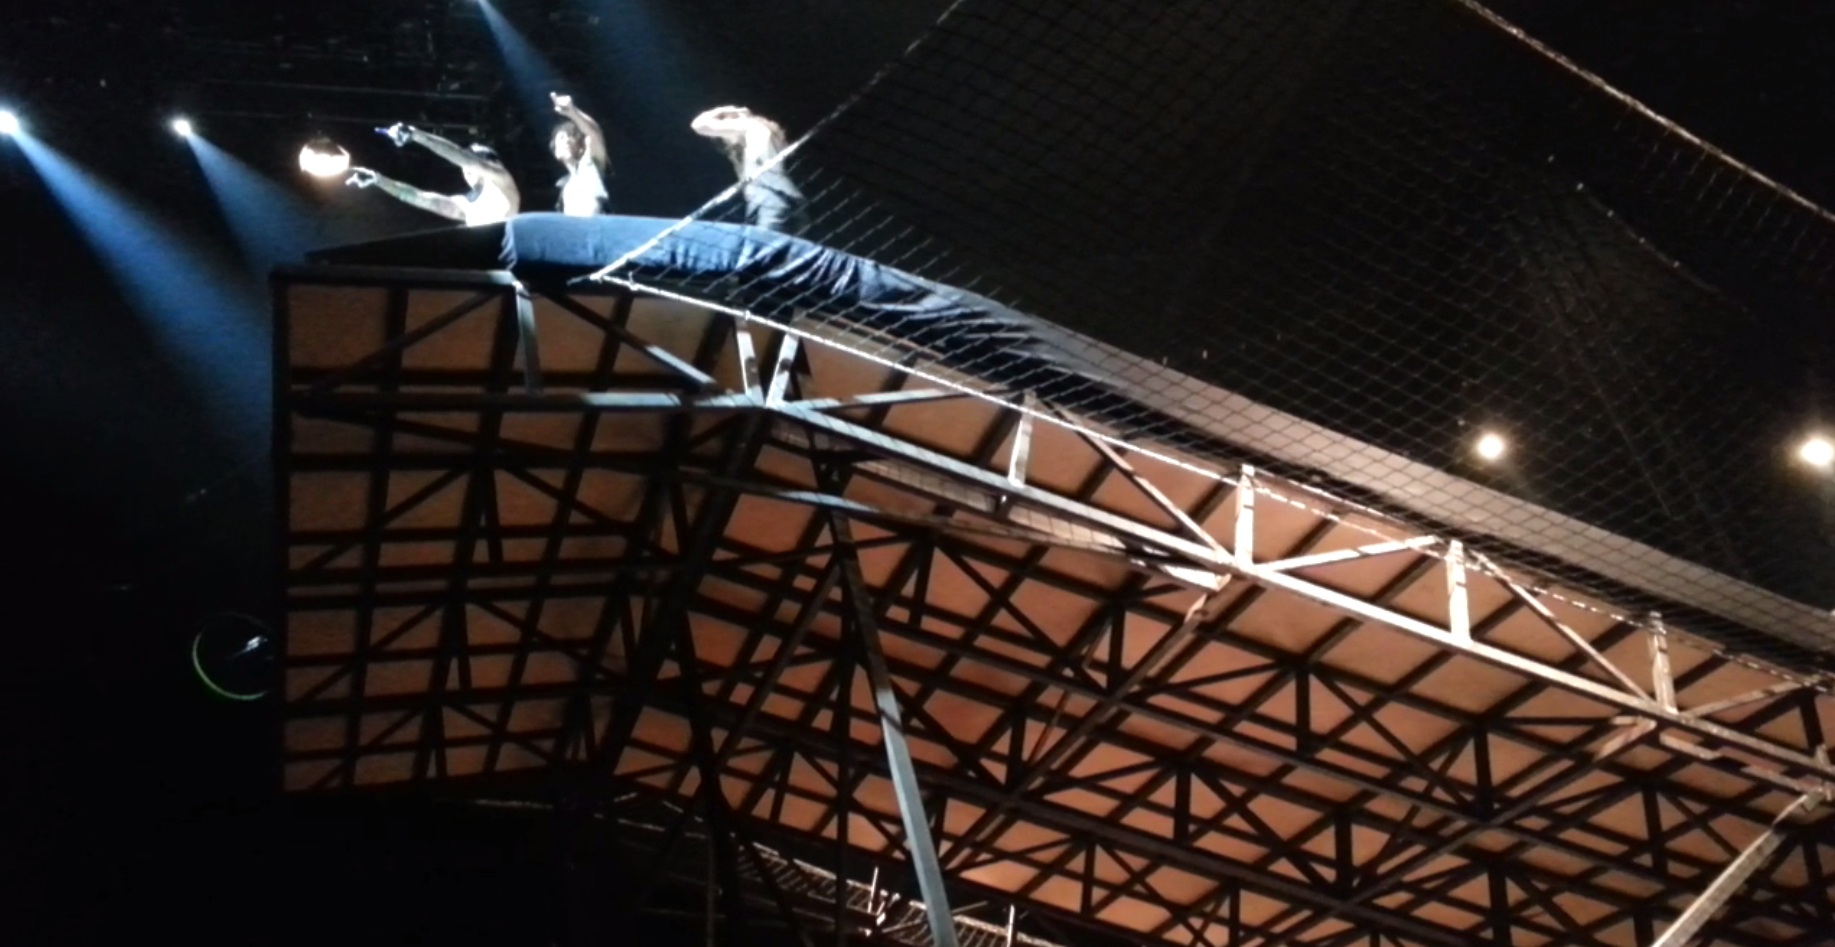
\includegraphics[width=.335\textwidth]{./gfx/400_UGV_Quality/Video_Frames/Bike3}
		\\ 
		\multicolumn{3}{c}{Video sequence: Sports 2}\\
		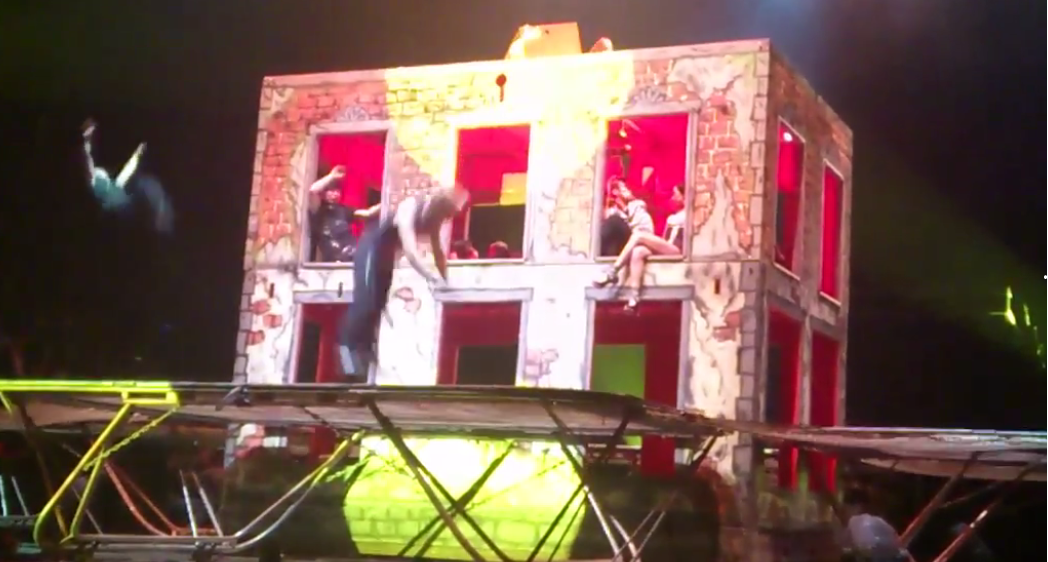
\includegraphics[width=.315\textwidth]{./gfx/400_UGV_Quality/Video_Frames/jump1} &
		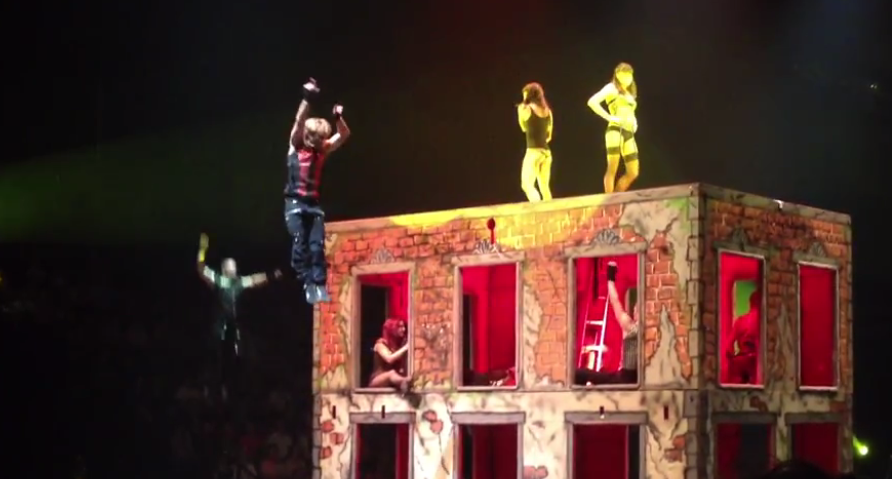
\includegraphics[width=.315\textwidth]{./gfx/400_UGV_Quality/Video_Frames/jump2} &
		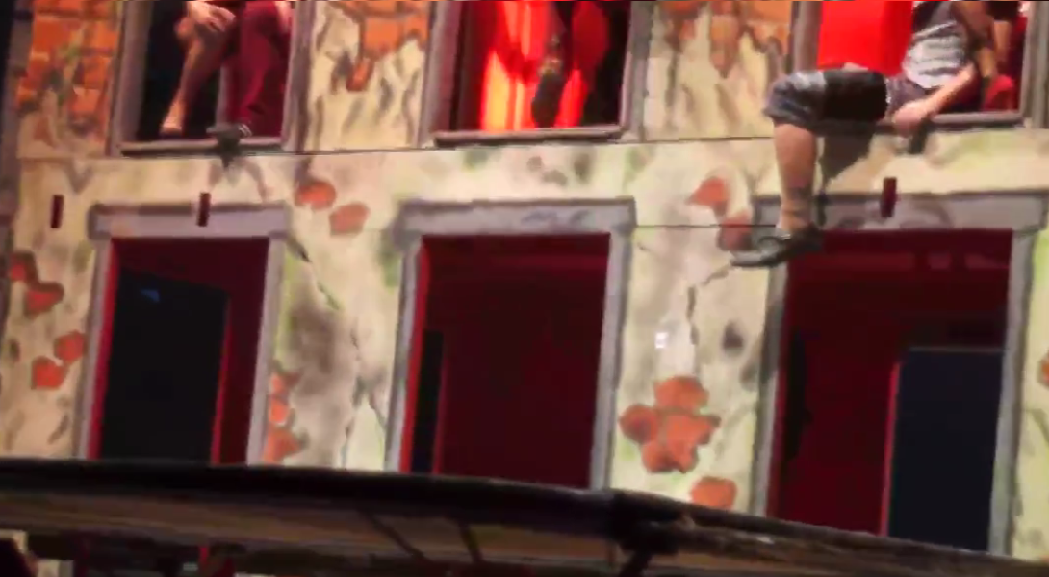
\includegraphics[width=.3\textwidth]{./gfx/400_UGV_Quality/Video_Frames/jump3}
		\\ 
		\multicolumn{3}{c}{Video sequence: Show 1}
		\\
		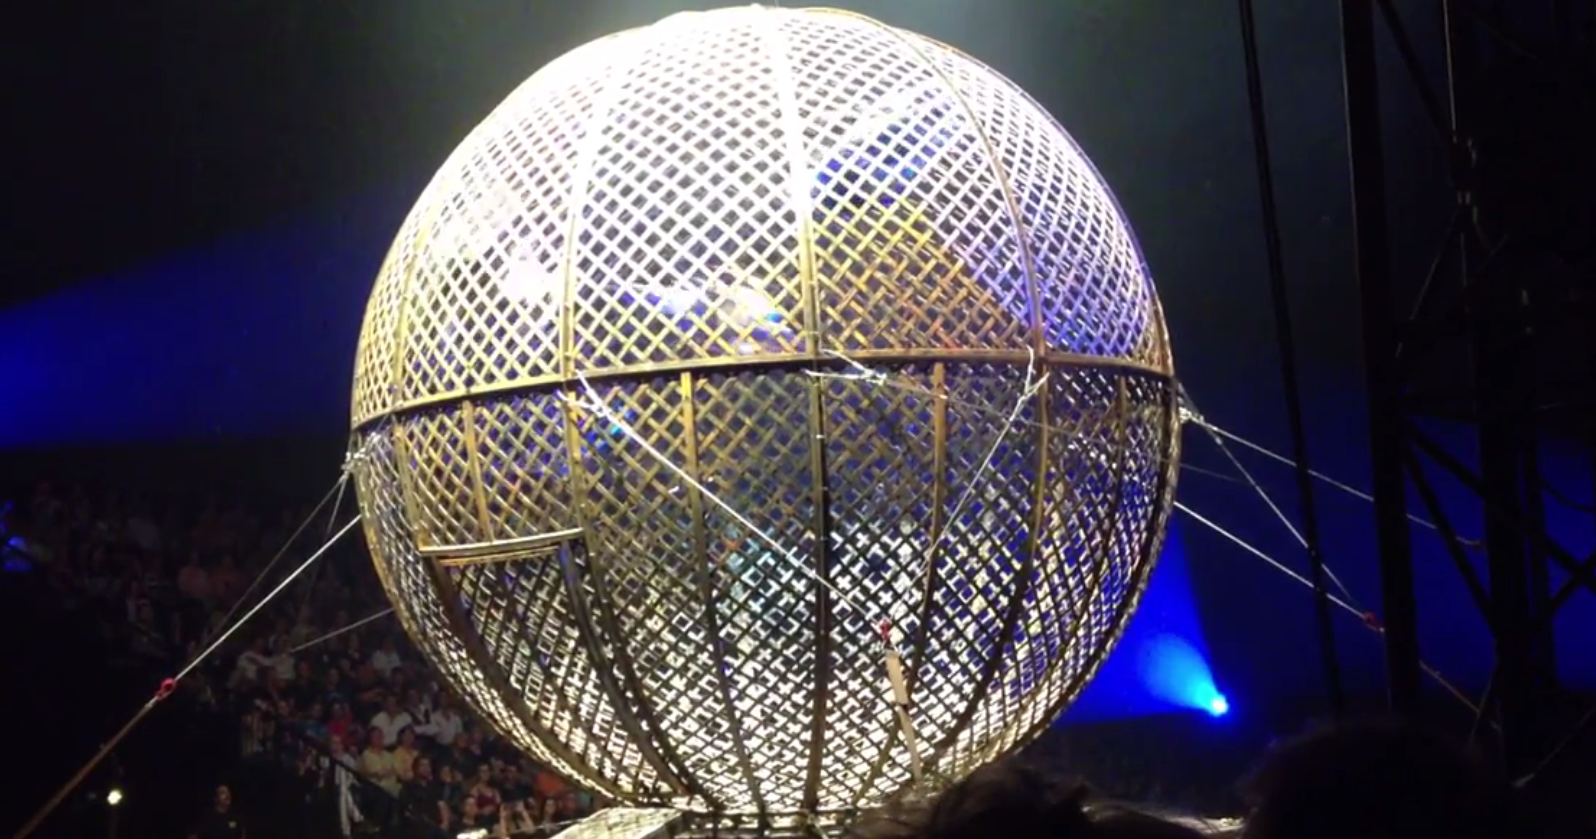
\includegraphics[width=.31\textwidth]{./gfx/400_UGV_Quality/Video_Frames/motor_circle_1} &
		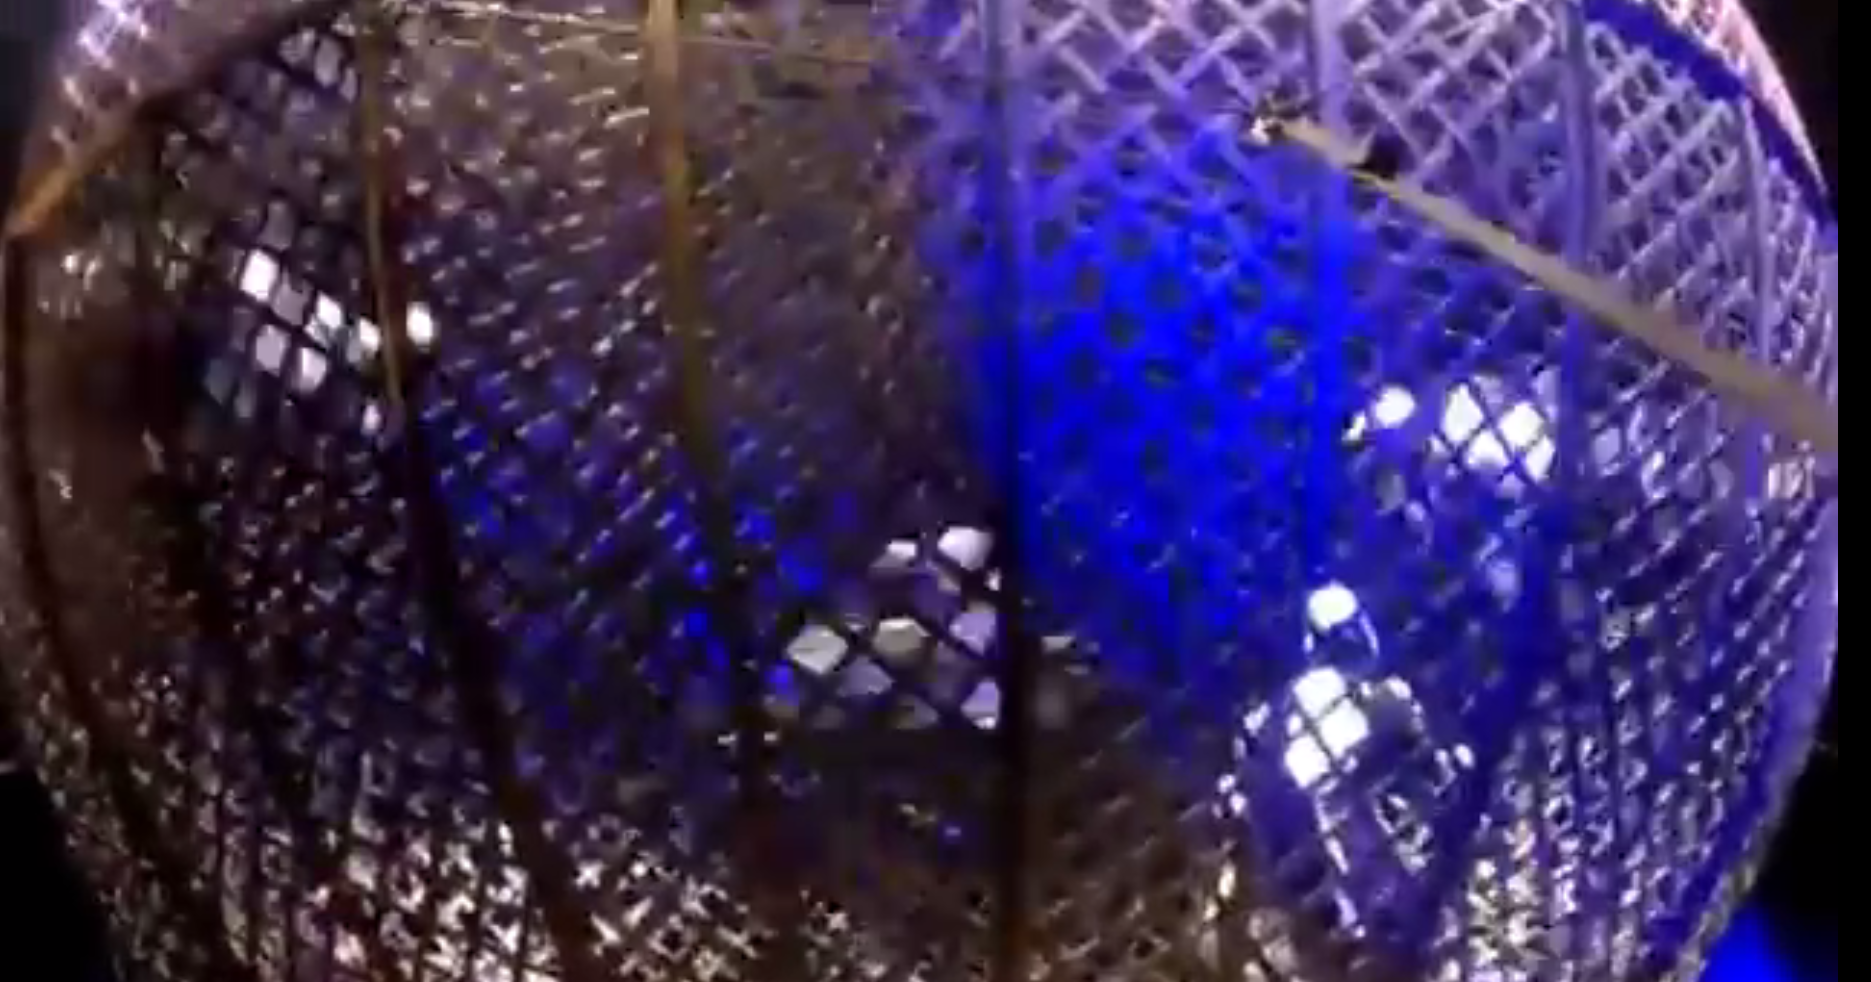
\includegraphics[width=.31\textwidth]{./gfx/400_UGV_Quality/Video_Frames/motor_circle_2} &
		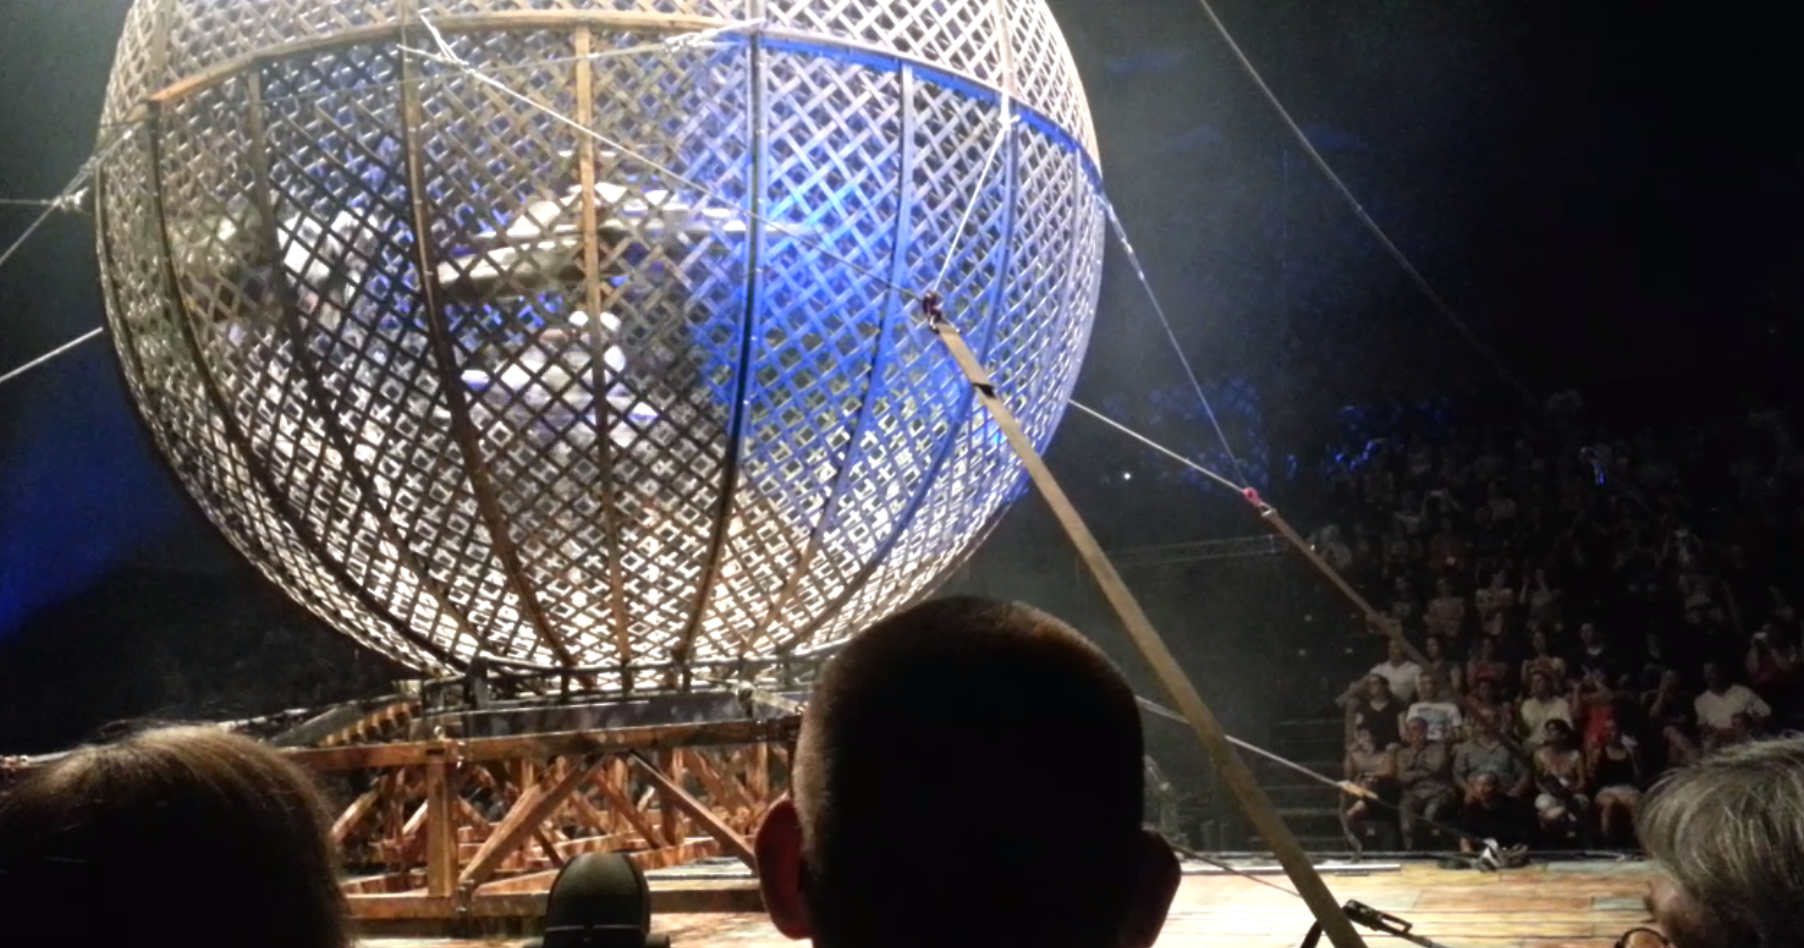
\includegraphics[width=.31\textwidth]{./gfx/400_UGV_Quality/Video_Frames/motor_circle_3}
		\\ 
		\multicolumn{3}{c}{Video sequence: Show 2}
		
		
	\end{tabular}
	\caption[Sample frames for the recording position dataset.]{Impressions of the video datasets used to evaluate the perceived quality based on the recording position.}
	\label{fig:420_impression}
\end{figure}

Examples of the videos are shown in Figure~\ref{fig:420_impression}.
"Show" and "sports" videos have been recorded during live performances in Darmstadt and Frankfurt, Germany. 
The videos include a circus comedy event ("Show 1"), an artistic performance, including rapid movements due to jumps ("Show 2"), and a concert with a crowded audience ("Music"). 
Sports events recorded include a soccer game ("Sports 1") and a motorbike competition, including jumps ("Sports 2"). 

All recordings contain a collaboratively determined \ac{RoI}, which differs regarding the viewing angle, distance - and thus the perceivable level of detail. 
Scenery sequences are taken in Paris, France showing the Eiffel Tower in different views ("Scenery 1"), in Darmstadt showing a historic building ("Scenery 2") and another \ac{PoI} in Darmstadt ("Scenery 3").  
Similar to the videos used in the recording quality assessment, all video sequences have a duration between 9 and 12 seconds. 
Audio tracks are removed from the videos. 
Video sequences are compressed at their recording and have a resolution of \ac{4CIF} similar to the other study. 
